\documentclass{beamer}
\usepackage[spanish, english]{babel}
\selectlanguage{spanish}
\usepackage[fixlanguage]{babelbib}
\selectbiblanguage{spanish}
\usepackage{graphicx}
\usepackage[utf8]{inputenc}%Para poder usar acentos y otras letras latinas del español
\usepackage[T1]{fontenc}
\usepackage{verbatim}%comments

\usepackage{caption, subcaption}

\bibliographystyle{bababbrv}

\usetheme{Darmstadt}

\title{Clasificación de Razas}
\subtitle{De Perros y Gatos}


\author[Bahamonde, Gonz\'alez]{J.~Bahamonde\inst{1} \and S.~Gonz\'alez\inst{1}}
\institute[University de Chile]
{
	\inst{1}
	Departamento de las Ciencias de la Computaci\'on\\
	Universidad de Chile
}

\begin{document}
	\frame{\titlepage}
	\begin{frame}{¿Cuál es el problema?}
		\begin{itemize}
			\item{
				Detección de múltiples rostros animales.\\
				{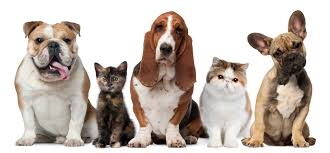
\includegraphics[scale=0.3]{imagen/catsydogs.jpg}}
			}
			\item{
				Reconocimiento de raza de animales.\\
				{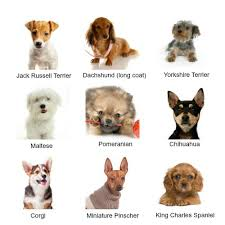
\includegraphics[scale=0.6]{imagen/doguebreed.jpg}}
			}
		\end{itemize}
	\end{frame}
	\begin{frame}{¿Cuál es el problema?}
		%CONTENT
		\begin{itemize}
			\item{
				El problema de clasificación entre clases muy disimilares ha sido ampliamente estudiado.
			}
			\item{
				El dataset Caltech presenta el problema de discriminar el Golden Gate con una iguana.
			}
			\item{
				Discriminar entre clases de perros, gatos, aves y flores es un problema de \textbf{Categorización fina de objetos} \textit{(fine  grained  object  categorization)}.
			}
		\end{itemize}
        \begin{center}
            {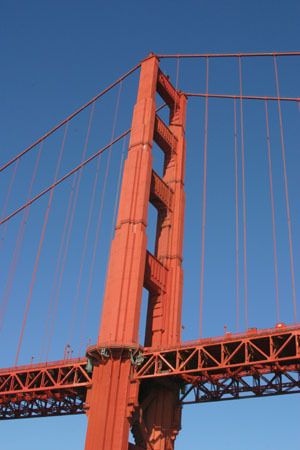
\includegraphics[scale=0.2]{imagen/ggate.jpg}}
    		{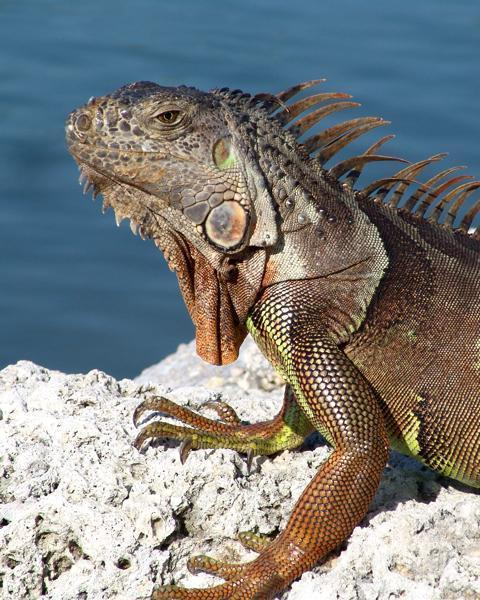
\includegraphics[scale=0.14]{imagen/iguana.jpg}}
        \end{center}

	\end{frame}
	\begin{frame}
		\frametitle{¿Cuál es el problema?}
		%CONTENT
		\begin{itemize}
			\item Las razas de animales pueden diferir en pequeñas características fenoitípicas.
			\item Los animales tienen formas altamente deformables.
		\end{itemize}
        \begin{center}
    		{
\includegraphics[scale=0.2]{imagen/fitsisits.jpg}}
	    	{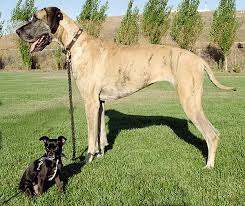
\includegraphics[scale=0.5]{imagen/dogdiff.jpg}}
        \end{center}
	\end{frame}
	\begin{frame}{Aplicación}
		\begin{itemize}
			\item{El problema es similar a la clasificación de Aves.\\
			Ej. Monitorear automáticamente la población de aves, de una determinada especie, en un parque forestal.\\
			}
			\item{También es similar a la clasificación de  flores.\\
			Ej. Determinar la especie de una flor a partir de su fotografía, puede servir a herboristas en el campo.
			}
			\item{La detección automática de razas de animales, puede servir de apoyo a veterinarios, o a buscar animales perdidos.\\
			}
		\end{itemize}
	\end{frame}
	\begin{frame}{Propuesta de solución}
\begin{itemize}
\item{
		Entrenar un modelo con HOG
}
\item{
		Alinear por orejas: Extraer información de Forma
}
\item{
		Alinear por ojos: Extraer información de Textura
}
\item{
		Utilizar un descriptor de color.
}
\end{itemize}
	\end{frame}
	\begin{frame}{Función de nuestra solución}
		Dado una imagen de consulta, en la que el rostro del animal ya ha sido detectado y etiquetado, es decir, están identificados los ojos, nariz, orejas, se determinará la especie y raza a la que pertenesca. 
	\end{frame}

    \begin{frame}{Estado del Arte: Gatos y Perros \footnote{\emph{Cats and
        Dogs}, Parkhi, Vedaldi, Zisserman y Jawahar, 2012.}}
        \begin{itemize}
            \item Modelo de partes deformables (HOG + resortes).
            \item \emph{Bag-of-words} con descriptores SIFT. 
            \item Segmentación automática mediante \emph{grab-cut}.
        \end{itemize}
        \begin{center}
            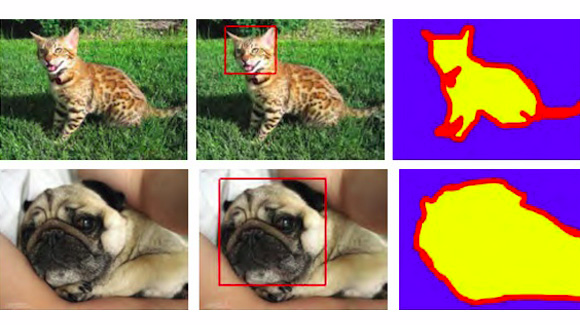
\includegraphics[scale=0.3]{imagen/catsanddogs_annotation}
        \end{center}
	\end{frame}

    \begin{frame}{Estado del Arte: Clasificación de Razas de
            Perros\footnote{\emph{Dog Breed Classification Using Part
        Localization}, Liu, Kanazawa, Jacobs y Belhumeur, 2012. }}
        \begin{itemize}
            \item Detección de cara del perro.
            \item Identificación de partes.
            \item Histograma de color y descriptores SIFT en torno a las partes.
        \end{itemize}
        \begin{center}
            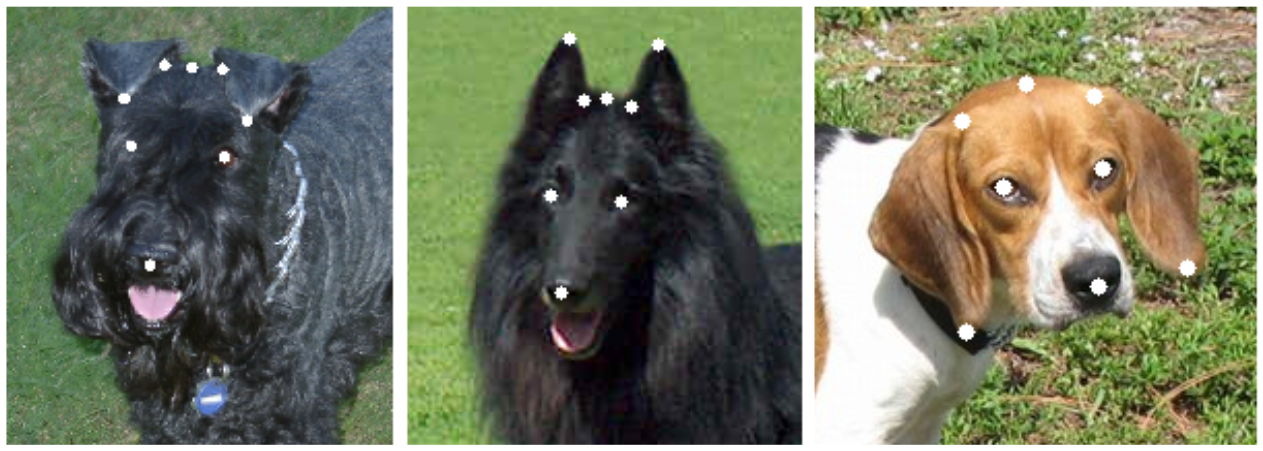
\includegraphics[scale=0.15]{imagen/dogannotation}
        \end{center}
	\end{frame}
    \begin{frame}{Estado del Arte: Detección de Gatos \footnote{\emph{Cat Head
        Detection - How to Effectively Exploit Shape and Texture Features},
Zhang, Sun, Tang, 2008}}
        \begin{itemize}
            \item No es clasificación, sino que detección.
            \item Entrenan dos detectores con \emph{datasets} normalizados de
                distinta forma.
            \item Un clasificador fusiona la información de ambos para decidir
                si está frente a un gato o no.
        \end{itemize}
        \begin{center}
            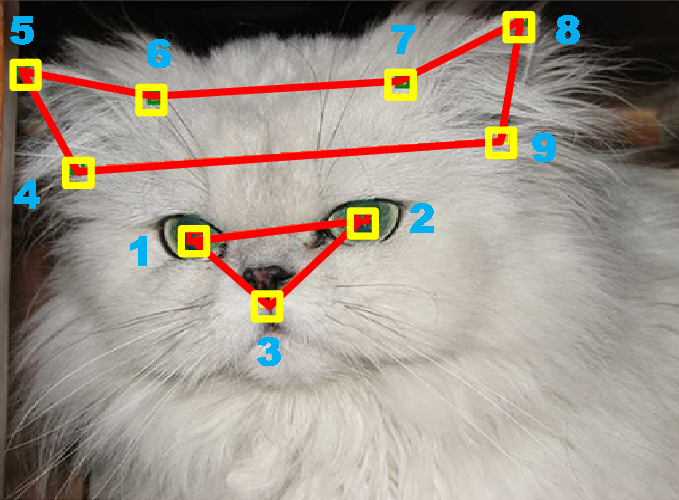
\includegraphics[scale=0.25]{imagen/annotation}
        \end{center}
    \end{frame}

	\begin{frame}{Nuestra aproximación}
		Trabajaremos sobre imágenes en las que los rostros de los animales ya ha sido anotada.\\
		Buscamos describir al animal por su textura, forma y color.
	\end{frame}
	\begin{frame}{Innovaciones}
		Para trabajar con perros hay que crear un dataset anotando los ojos, nariz y orejas.
		Ya que necesitamos alinear los perros para extraer forma.
	\end{frame}
	\begin{frame}{Evaluación}
		Para determinar el desempeño de la clasificación usaremos una matriz de confusión.
	\end{frame}
%COMENTARIO INICIA ACA=================================================================================================
\begin{comment}

	\begin{frame}
		\frametitle{Estado del Arte.}
		%CONTENT
		\selectlanguage{spanish}
		\selectbiblanguage{spanish}
		\bibliography{./presentation}
	\end{frame}
	\begin{frame}
		\frametitle{Reconocimiento facial de gatos.}
		%CONTENT
		\url{http://harthur.github.io/kittydar/}

		Utiliza método propuesto en \emph{Cat head detection-how to effectively exploit shape and texture features}\cite{zhang2008cat}
		\begin{figure}[H]
			\centering
			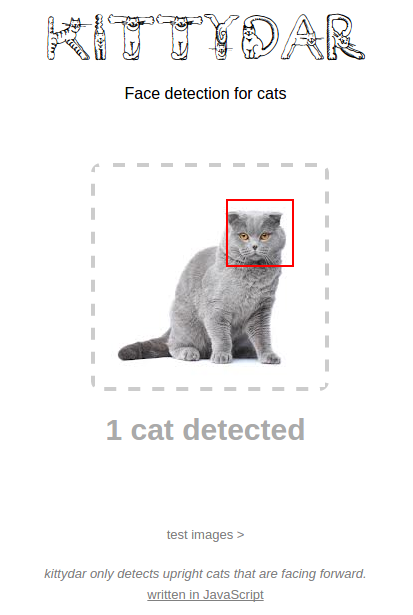
\includegraphics[scale=0.27]{imagen/Captura.png}
		\end{figure}
	\end{frame}
	\begin{frame}
		\frametitle{Reconocimiento facial de gatos.}
		%CONTENT
		Comparación entre métodos.
		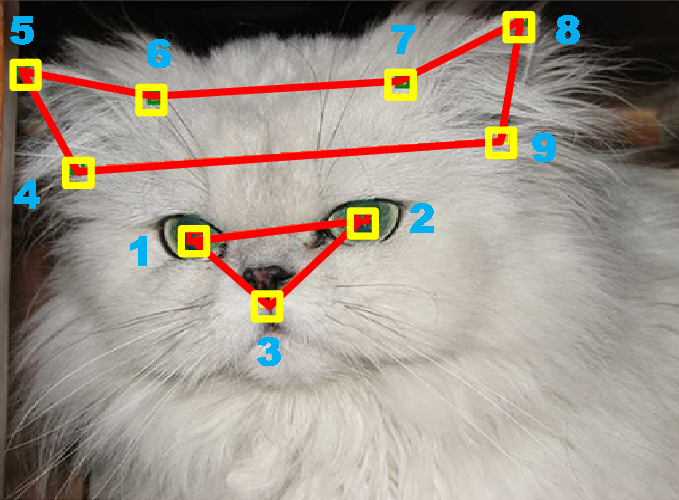
\includegraphics[scale=0.15]{imagen/annotation.png}
		\begin{itemize}
			\item{
				HOG.
			}
			\item{
				Haar.
			}
			\item{
				Detección de formas y textura conjunta.
			}
		\end{itemize}
		\begin{figure}[H]
			\centering
			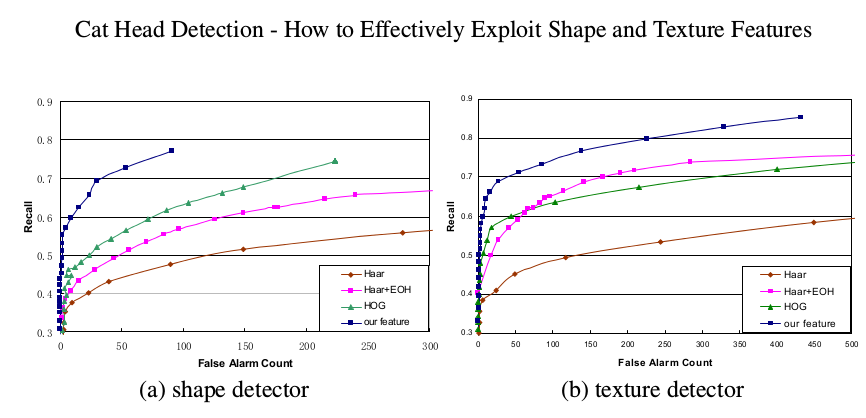
\includegraphics[scale=0.30]{imagen/cat-roc.png}
		\end{figure}
	\end{frame}
	\begin{frame}
		\frametitle{Resultados}
		%CONTENT
		\begin{figure}[H]
			\centering
			\subcaptionbox{}{
\includegraphics[scale=0.07]{imagen/nw1.jpg}}
			\subcaptionbox{}{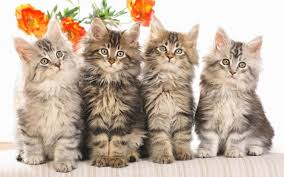
\includegraphics[scale=0.38]{imagen/nw2.jpg}}
			\subcaptionbox{}{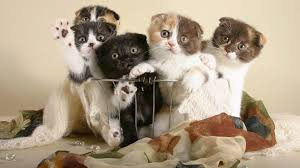
\includegraphics[scale=0.39]{imagen/nw3.jpg}}
			\caption{No reconoce gatitos.}
		\end{figure}
	\end{frame}
	\begin{frame}
		\frametitle{Resultados}
		%CONTENT
		\begin{figure}[H]
			\centering
			\subcaptionbox{}{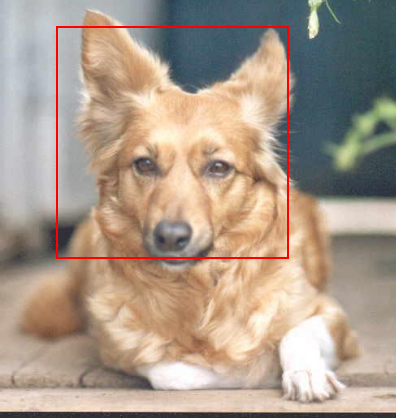
\includegraphics[scale=0.3]{imagen/w1.png}}
			\subcaptionbox{}{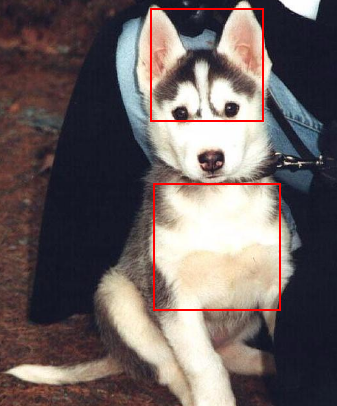
\includegraphics[scale=0.31]{imagen/w2.png}}
			\caption{Reconoce algunos perros.}
		\end{figure}
	\end{frame}
	\begin{frame}
		\frametitle{Resultados}
		%CONTENT
		\begin{figure}[H]
			\centering
			\subcaptionbox{}{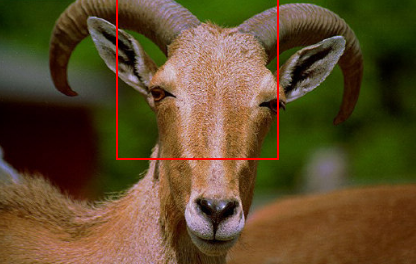
\includegraphics[scale=0.27]{imagen/f1.png}}
			\subcaptionbox{}{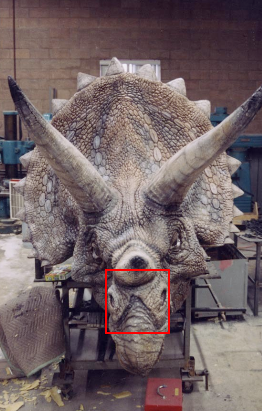
\includegraphics[scale=0.28]{imagen/f2.png}}
			\subcaptionbox{}{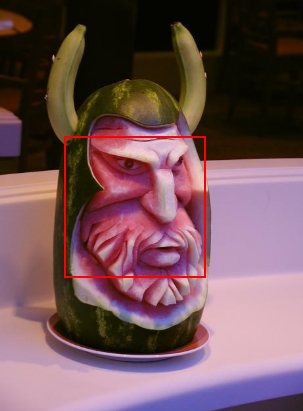
\includegraphics[scale=0.28]{imagen/f3.png}}
			\caption{Reconoce... cosas.}
		\end{figure}
	\end{frame}
	\begin{frame}
		\frametitle{Clasificación en Razas de Gatos y Perros.}
		%CONTENT
		\emph{Cats and Dogs}.\cite{parkhi12a}
		\begin{itemize}
			\item{
				HOG para reconocimiento de \emph{Forma}.
			}
			\item{
				\emph{Bag of Words} para reconocimiento de \emph{textura}.
			}
		\end{itemize}
		Combinaciones de Rostro, Cuerpo y Fondo.
		\begin{figure}[H]
			\centering
			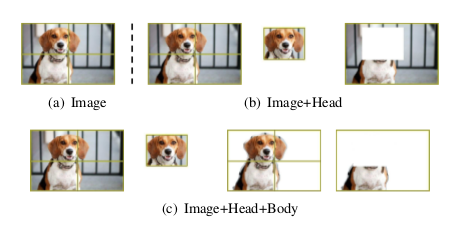
\includegraphics[scale=0.50]{imagen/faceheadimage.png}
		\end{figure}
	\end{frame}
	\begin{frame}
		\frametitle{Clasificación en Razas de Gatos y Perros.}
		%CONTENT
		\begin{figure}[H]
			\centering
			{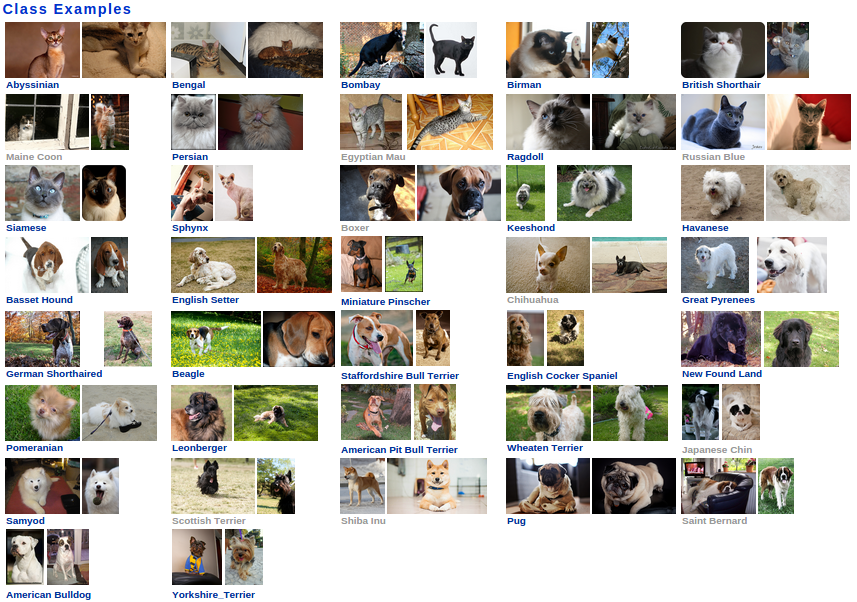
\includegraphics[scale=0.27]{imagen/datasetEx.png}}
			\caption{Dataset de razas de Perros y Gatos.}
		\end{figure}
	\end{frame}
	\begin{frame}
		\frametitle{Reconocimiento facial de Perros.}
		%CONTENT
		\emph{Biometric Recognition for Pet Animal}.\cite{kumar2014biometric}

		PCA \& Eigenfaces.
	\end{frame}
	\begin{frame}
		\frametitle{Reconocimiento facial de Perros.}
		%CONTENT
		\begin{figure}[H]
			\centering
			{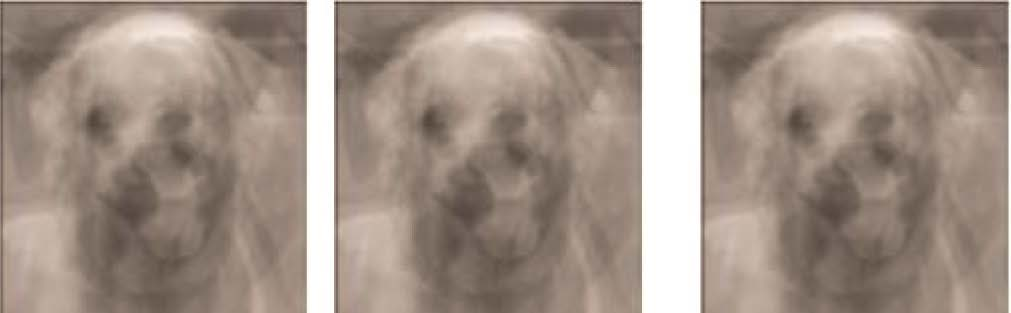
\includegraphics[scale=0.27]{imagen/dogaverage.png}}
			\caption{Eigenfaces para Perros.}
		\end{figure}
	\end{frame}

%COMENTARIO TERMINA ACA ==============================================================================
\end{comment}
\end{document}
